\documentclass{article}[12pt]
\usepackage{color}
\usepackage[normalem]{ulem}
\usepackage{times}
\usepackage{fullpage}
\usepackage{amsmath}
\usepackage{amssymb}
\usepackage{tikz}
\def \R {\mathbb R}
\def \imp {\Longrightarrow}
\def \eps {\varepsilon}
\def \Inf {{\sf Inf}}
\newenvironment{proof}{{\bf Proof.  }}{\hfill$\Box$}
\newtheorem{theorem}{Theorem}[section]
\newtheorem{definition}{Definition}[section]
\newtheorem{corollary}{Corollary}[section]
\newtheorem{lemma}{Lemma}[section]
\newtheorem{claim}{Claim}[section]
\setlength {\parskip}{2pt}
\setlength{\parindent}{0pt}

\newcommand{\headings}[4]{\noindent {\bf Assignment 2 CME241} \hfill {{\bf Author:} Nicolas Sanchez} \\
{} \hfill {{\bf Due Date:} #2} \\

\rule[0.1in]{\textwidth}{0.025in}
}

\newcommand{\klnote}[1]{{\color{red} #1}}
\newcommand{\klsout}[1]{{\color{red} \sout{#1}}}

\begin{document}

\headings{\#1}{Tuesday, October 8, 10:30am}\section{} 



\section{Manual Value Iteration}
We do the steps of value iteration.
\begin{align*}
v_1(s_1) &= \max\{q_1(s_1,a_1), q_1(s_1,a_2)\} = \max\{ 8 + (0.2*10 + 0.6*1.0), 10+(0.1*10+0.2*1)\} = \max\{10.6, 11.2\} = 11.\\
v_1(s_2) &= \max\{q_1(s_1,a_1), q_1(s_1,a_2)\} =   \max\{ 1+ (0.3*10 + 0.3*1.0),-1+(0.5*10+0.3*1)\} = \max\{4.3, 4.3\} = 4.3\\
\pi_1(s_1) &= a_2\\
\pi_1(s_2) &= a_1\\
v_1(s_1)  &= \max\{ 8 + (0.2*11.2 + 0.6*4.3), 10+(0.1*11.2+0.2*4.3)\} = \max\{12.82, 11.98\} = 12.82\\
v_1(s_2) &= \max\{ 1+ (0.3*11.2 + 0.3*4.3), -1+(0.5*11.2+0.3*4.3)\} = \max\{5.65, 5.89\} = 5.89\\
\pi_2(s_1) &= a_1\\
\pi_2(s_2) &= a_2\\
\end{align*}
We now notice that by construction, that the difference between action $a_1$ and $a_2$ for state $s_1$ grows if the values grow, or specifically $q_k(s_1,a_1) - q_k(s_1,a_2) > q_{k-1}(s_1,a_1) - q_{k-1}(s_1,a_2)$ if $v_k(s) > v_{k-1}(s) $ because of the strictly higher likelihoods to go to each of these states. Since only the transition probs are all positive, the values of the states will monotonically increase, meaning we will always have $q_k(s_1,a_1) > q_k(s_1,a_2)$. An analogous argument works for  $q_k(s_2,a_2) > q_k(s_2,a_1)$ and leaves us with the optimal policy:
\begin{align*}
\pi(s_1) &= a_1\\
\pi(s_2) &= a_2\\
\end{align*}
\section{Frog Croaking Revisited}

Both policy and value iteration are orders and orders of magnitude faster than the exhaustive grid search. Indeed for 25 lilypads, value iteration takes 120 iteration and policy iteration takes 4 vs the 33mm possible policies in the exhaustive search. Interestingly the limited number of actions as well as the symmetric aspect of the problem for anything not at the beginning of the track means that policy iteration actually does not take longer to converge as the problem grows bigger.

\begin{figure}
  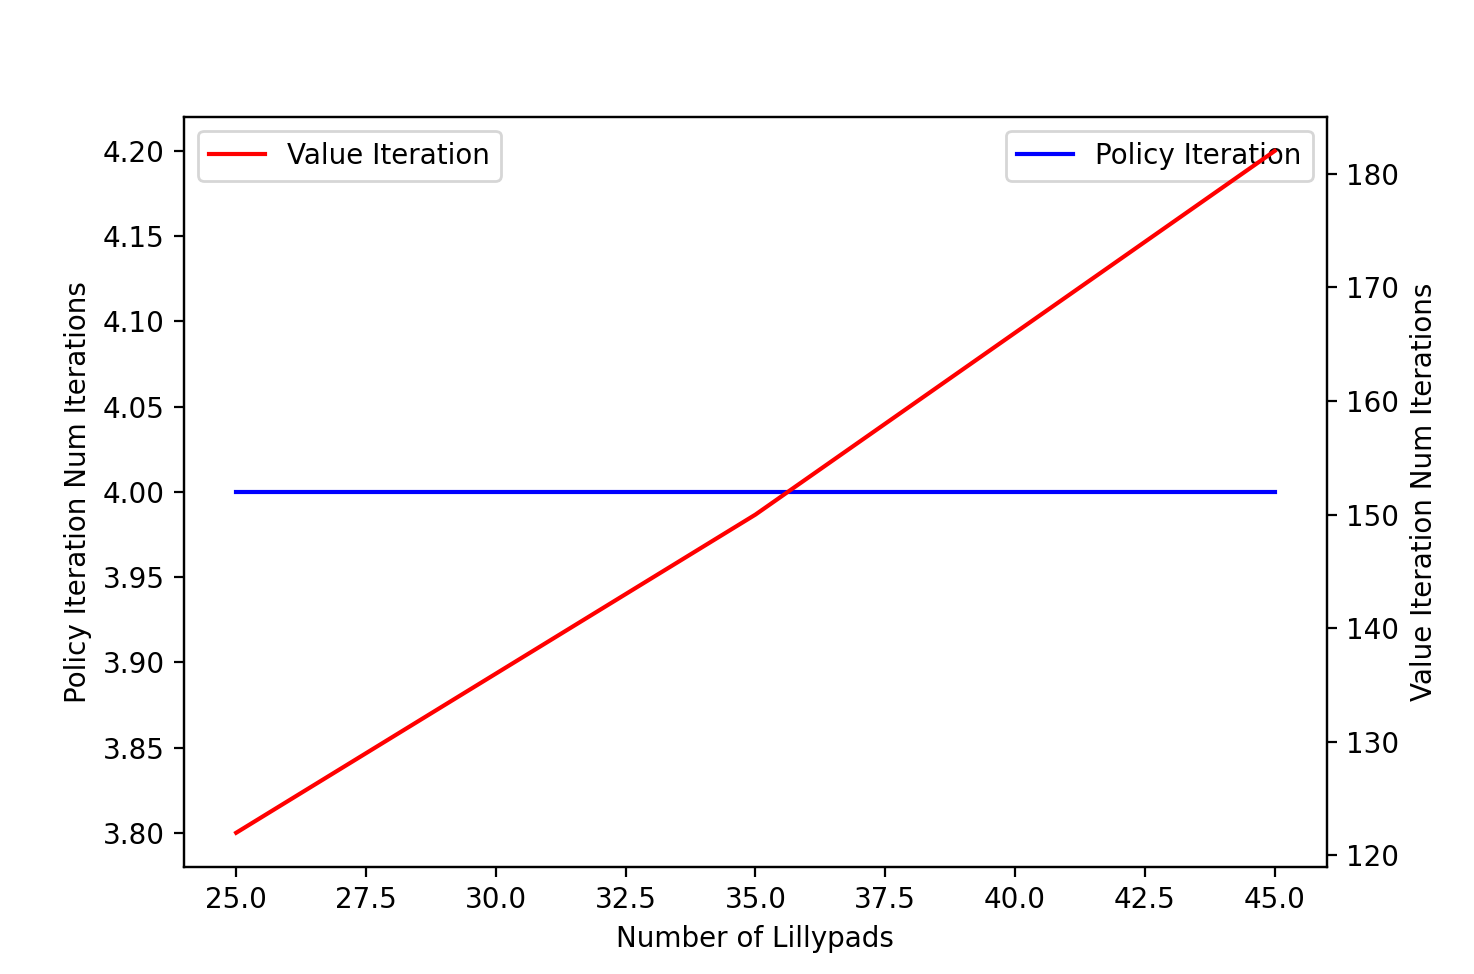
\includegraphics[width=\linewidth]{CovergenceSpeed.png}
  \caption{Iterations needed for convergence}
  \label{fig:llp3}
\end{figure}

\section{Job Hopping and Wages-Utility Maximisation}
The state will be a tuple $s_t = (s,i)$ with $s\in\{\tilde{e}, \tilde{u}\}$ and $i \in [1,2,\ldots,n]$.\\
The action space will be:
\begin{align*}
A_t(s,i) = \begin{cases} \{A\} \text{ if $s = \tilde{e}$} \\ \{A, R\} \text{ if $s=\tilde{u}$}\end{cases}
\end{align*}
The transition probabilities will be as follows:
\begin{align*}
P((s,i), A, (\tilde{e},j) &= (1-\alpha)\delta_{ij}\\
P((s,i), A, (\tilde{u},j) &= \frac{\alpha}{n}\\
P((\tilde{u},i), R, (\tilde{u},j) &= \frac{1}{n}\\
\end{align*}
With all other transition probabilities being zero. The reward function is:
\begin{align*}
R((\tilde{e},i), A, (s,j)) = \log(w_i)\\
R((\tilde{u},i), A, (\tilde{e},j) = \log(w_j)\\
R((\tilde{u},i), R, (s,j) = \log(w_0)\\
\end{align*}

This yields the following Bellman equations:
\begin{align*}
V(\tilde{e}, i) &= \log(w_i) + (1-\alpha)\gamma V(\tilde{e},i) + \frac{\alpha\gamma}{n} \sum_{j=1}^n V(\tilde{u}, j)\\
V(\tilde{u}, i) &= \max\{\log(w_i) + (1-\alpha)\gamma V(\tilde{e},i) + \frac{\gamma\alpha}{n} \sum_{j=1}^n V(\tilde{u}, j), \log(w_0)+ \frac{\gamma}{n} \sum_{j=1}^n V(\tilde{u}, j)\}\\
\end{align*}
And we can rearrange these to get:
\begin{align*}
V(\tilde{e}, i) &= \frac{\log(w_i) + \frac{\alpha\gamma}{n} \sum_{j=1}^n V(\tilde{u}, j)}{1-\gamma(1-\alpha)}\\
V(\tilde{u}, i)& =  \max\{V(\tilde{e},i), \log(w_0)+ \frac{\gamma}{n} \sum_{j=1}^n V(\tilde{u}, j)\} \\
\end{align*}
Which one step further yields:
\begin{align*}
V(\tilde{e}, i) &= \frac{\log(w_i) + \frac{\alpha\gamma}{n} \sum_{j=1}^n V(\tilde{u}, j)}{1-\gamma(1-\alpha)}\\
V(\tilde{u}, i)& =  \max\{ \frac{\log(w_i) + \frac{\alpha\gamma}{n} \sum_{j=1}^n V(\tilde{u}, j)}{1-\gamma(1-\alpha)}, \log(w_0)+ \frac{\gamma}{n} \sum_{j=1}^n V(\tilde{u}, j)\} \\
\end{align*}

We can now hence implement an algorithm that repeatedly updates $V(\tilde{u}, i)$ and then once it converges, calculate the final $V(\tilde{e}, i)$. This is implemented in worker.py. The start point for $V(\tilde{u}, i)$ is the "worst case" scenario of being unemployed for ever: $\frac{1}{1-\gamma}{\log(w_0)}$.


\section{Lilypads on a Pond}
We set the state space to be the current location of the frog, aka the number of the lilypad and write out the action space for each non terminal state which is the same:
\begin{align*}
s_t \in \mathbf{S}& =\{0,\ldots n\}\\
\mathbf{T}& = \{n\}\\
A(s_t) &= \{\tilde{A},\tilde{B}\}
\end{align*} 

\begin{align*}
P(j | i, \tilde{A}) &=  \begin{cases} \frac{i}{n} \text{ if $j=i-1$}\\ \frac{n-i}{n} \text{ if $j=i+1$} \\ 0 \text{  otherwise} \end{cases}\\
P(j | i, \tilde{B}) &=  \begin{cases} 0 \text{ if $j=i$}\\ \frac{1}{n} \text{  otherwise} \end{cases}\\
\end{align*} 

In order to codify the benefit of escaping and detriment of being eaten we use the following reward function:
\begin{align*}
R(s,a,s') &=  \begin{cases} 1 \text{ if $s'=n$}\\ -1 \text{ if $s'=0$} \\ 0 \text{  otherwise} \end{cases}\\
\end{align*} 

We code this process up and obtain the following escape probabilities for $ n = 3,6,9$. We notice that the optimal policy seems to be to only croak B on the first step and otherwise croak A. This intuitively makes sense as for lily pad 1 both A and B give the same chance of going to lily pad 0 but at least croak B have a chance of advancing more than one step. For all other lily pads, croaking A instead of B gives you the same chance of advancing towards lilypad n but removes the chance of immediately going to lilypad 0.

\begin{figure}
  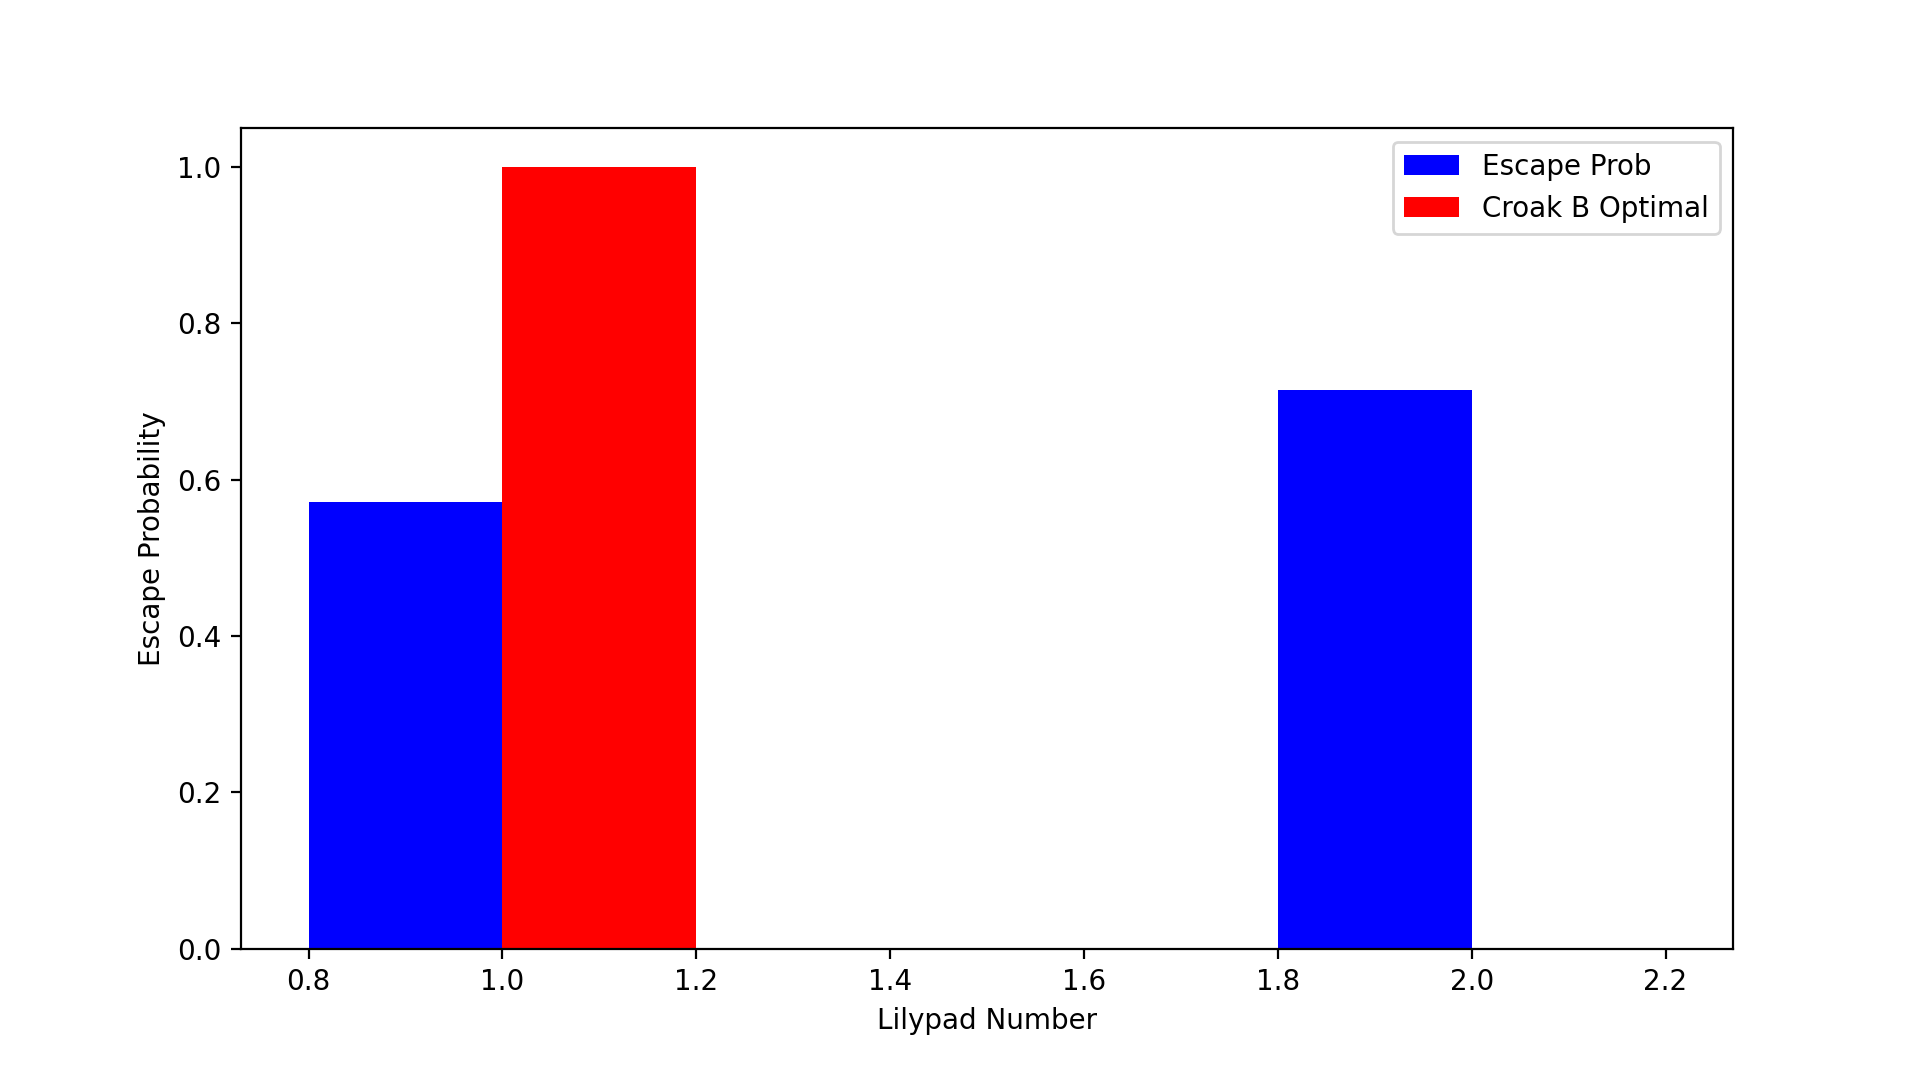
\includegraphics[width=\linewidth]{llp_3.png}
  \caption{Optimal Escape Probs and Optimal Policy}
  \label{fig:llp3}
\end{figure}

\begin{figure}
  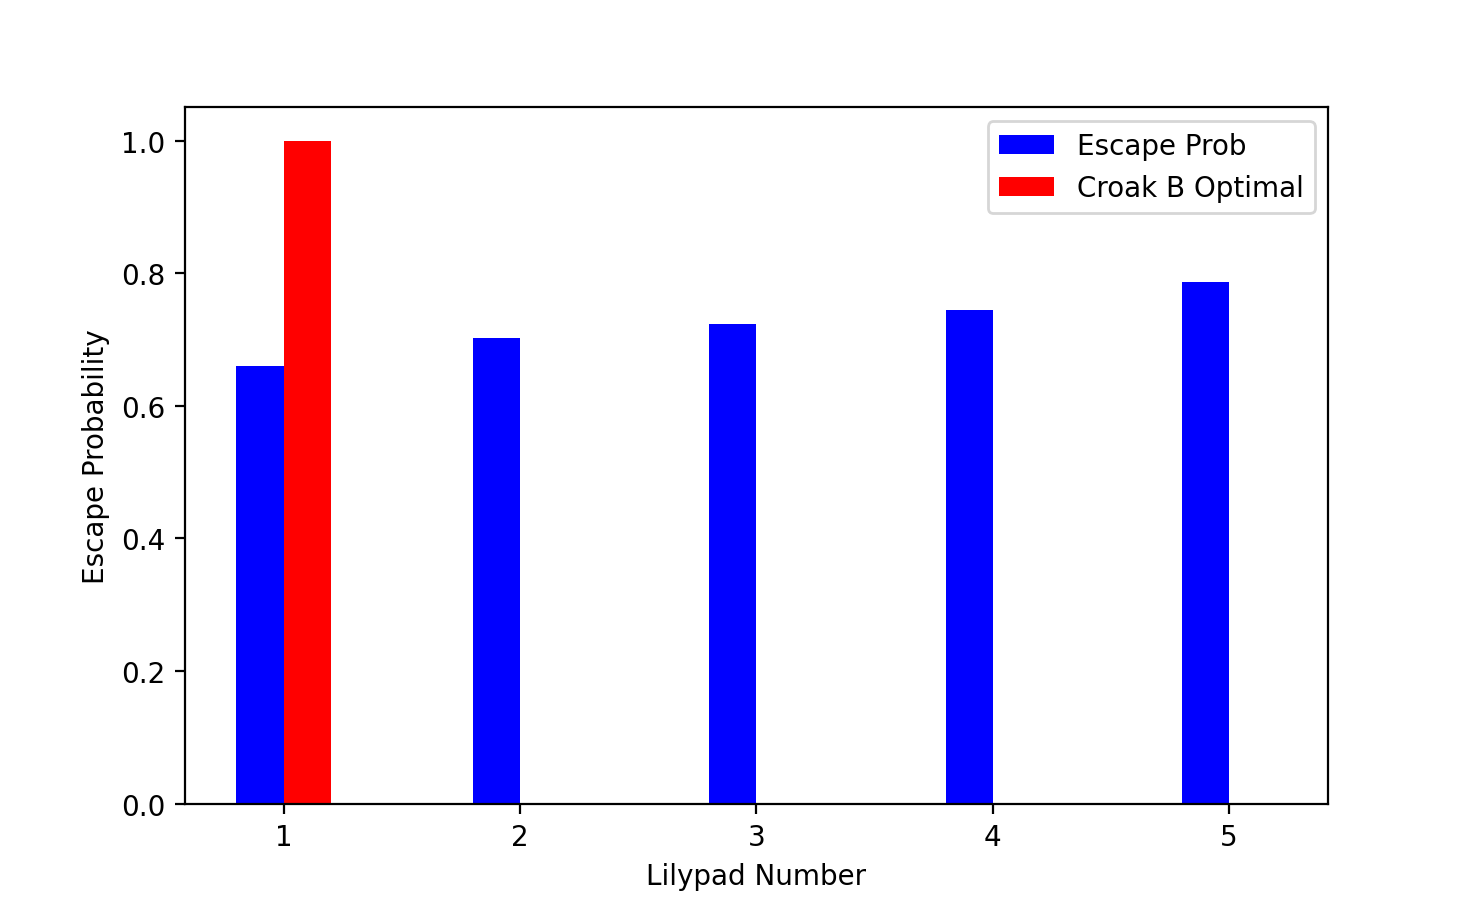
\includegraphics[width=\linewidth]{llp_6.png}
  \caption{Optimal Escape Probs and Optimal Policy}
  \label{fig:llp6}
\end{figure}

\begin{figure}
  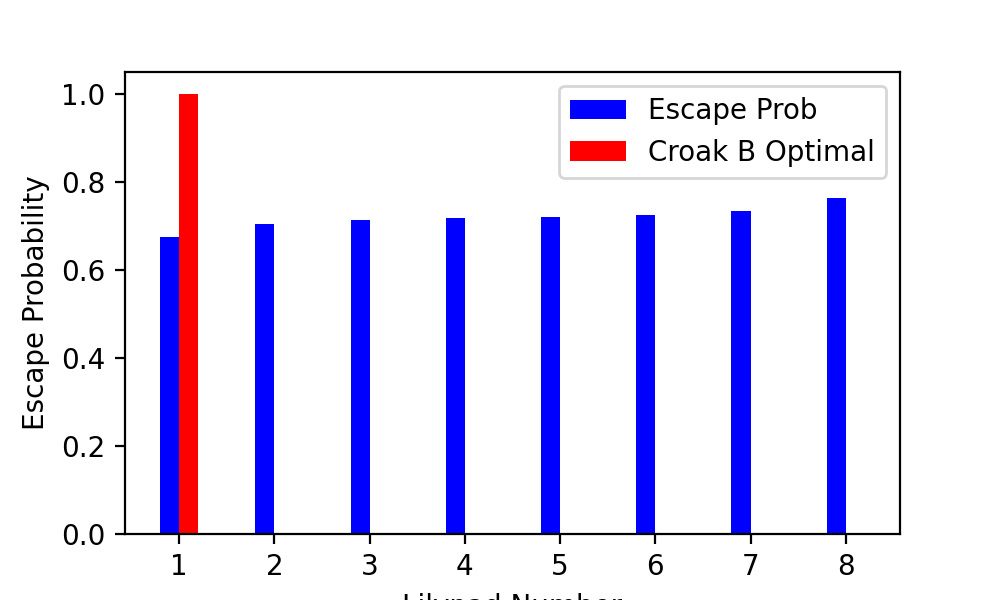
\includegraphics[width=\linewidth]{llp_8.png}
  \caption{Optimal Escape Probs and Optimal Policy}
  \label{fig:llp9}
\end{figure}

\section{Continuous Action Process}

We compute:
\begin{align*}
V(s) = E_s'[R(s') + 0V(s') | s,a] = E_s'-[e^{a,s'}]. = -M_x(a)
\end{align*}
In words, the cost function and transition probability means the value of a state is given by the negative of the moment generating function of a normal distribution of mean $s$ and variance $\sigma^2$ which is know to yield:
\begin{align*}
V(s) = e^{sa}e^{\frac{1}{2}\sigma^2 a^2}
\end{align*}
This quantity is minimized when its log is minimized so we must minimize $\frac{1}{2}\sigma^2a^2 + sa$ which is a quadratic expression known to obatin min at $a = \frac{-\sigma^2}{4s}$ yielding the the optimal value:
\begin{align*}
V^*(s) = e^{\frac{-\sigma^2}{4}}e^{\frac{1}{2}\sigma^2 \frac{-\sigma^4}{16s^2}} =  e^{\frac{-\sigma^2}{4}}e^{-\frac{1}{32} \frac{\sigma^6}{s^2}}
\end{align*}
\end{document}
